\begin{enumerate}[label=\thesection.\arabic*.,ref=\thesection.\theenumi]
\numberwithin{equation}{enumi}

\item The open loop tranfer function of a feedback system is 
\begin{align}
G(s)H(s) = \frac{s+3}{s^2(s-3)}
\label{eq:es17btech11009_system}
\end{align}
Find out how many times the Nyquist contour encircles $-1 + \j0$ in the clockwise direction.
\\
\solution The following code plots Fig. \ref{fig:es17btech11009_1}
%
\begin{figure}[!h]
\centering
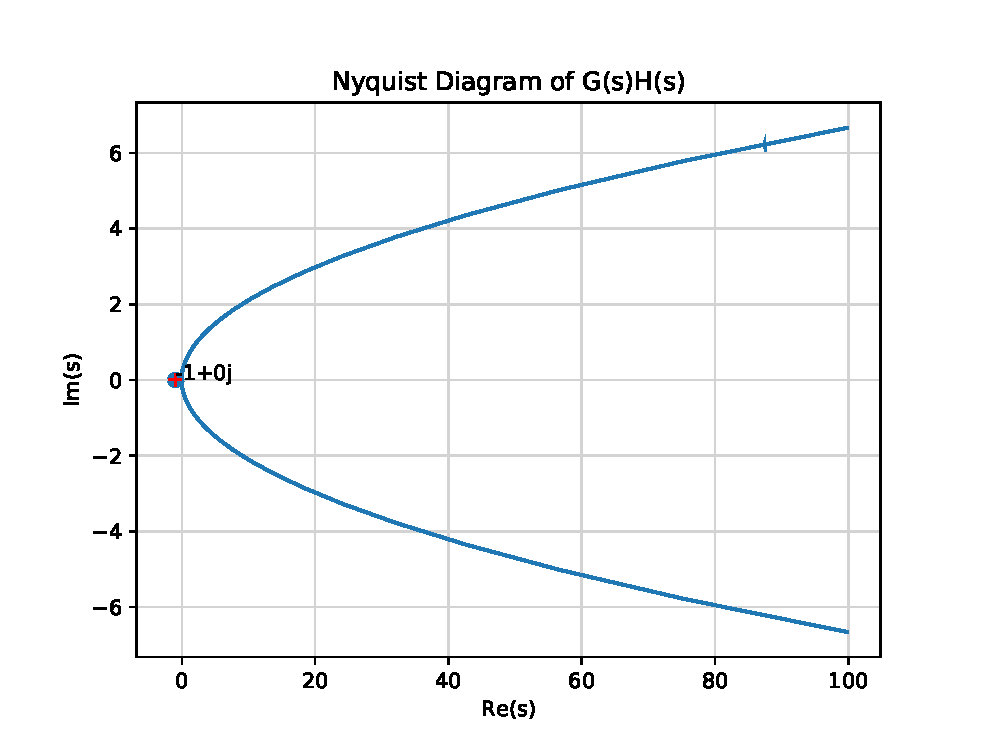
\includegraphics[width=\columnwidth]{./figs/es17btech11009.eps}
\caption{}
\label{fig:es17btech11009_1}
\end{figure}

\begin{lstlisting}
codes/es17btech11009.py
\end{lstlisting}
%
There is only one encirclement in the clockwise direction.
\end{enumerate}
